
\documentclass[letterpaper,twocolumn,10pt]{article}

% USENIX style file (2020-09 version as required by Security '26)
\usepackage{usenix-2020-09}

% Additional packages (url already in style file)
\usepackage{amsmath,amssymb,amsfonts}
\usepackage{graphicx}
\usepackage{booktabs}
\usepackage{pifont}

% Checkmark and X symbols
\newcommand{\cmark}{\ding{51}}
\newcommand{\xmark}{\ding{55}}
\newcommand{\pmark}{$\pm$}

% TikZ for architecture diagram
\usepackage{tikz}
\usetikzlibrary{arrows.meta,positioning,shapes.geometric,shapes.misc,fit,calc}

% Suppress microtype warning from USENIX style file
\makeatletter
\@ifpackageloaded{microtype}{\microtypecontext{spacing=nonfrench}}{}
\makeatother

%%%%%%%%%%%%%%%%%%%%%%%%%%%%%%%%%%%%%%%%%%%%%%%%%%%%%%%%%%%%%%%%%%%%%%%%%%%%%%%%
\begin{document}
%%%%%%%%%%%%%%%%%%%%%%%%%%%%%%%%%%%%%%%%%%%%%%%%%%%%%%%%%%%%%%%%%%%%%%%%%%%%%%%%

\title{SoK: Authorization in Multi-Agent Retrieval-Augmented Generation Systems}

\author{
{\rm Anonymous}\\
Anonymous Author
}

\maketitle

%%%%%%%%%%%%%%%%%%%%%%%%%%%%%%%%%%%%%%%%%%%%%%%%%%%%%%%%%%%%%%%%%%%%%%%%%%%%%%%%
\begin{abstract}
Retrieval-Augmented Generation (RAG) and multi-agent LLM systems are increasingly deployed in enterprise settings that handle sensitive data. While traditional software enforces least privilege via database predicates and API authorization, semantic retrieval and agent delegation introduce new authorization failure modes that are not captured by conventional access-control models.

This Systematization of Knowledge (SoK) paper organizes the authorization security landscape for agentic RAG. We (i) define a threat model and correctness criteria for authorization in semantic retrieval pipelines, (ii) develop a taxonomy of authorization failure modes including semantic overfetch, cross-domain synthesis leakage, and delegation escalation, (iii) classify and evaluate existing mitigation families such as role-partitioned indices, metadata-tag filtering, post-generation redaction, and agent tool-scope controls, and (iv) systematize a unifying correctness property, \emph{Authorization-First Retrieval (AFR)}, which treats authorization as a precondition to defining the semantic retrieval candidate space. AFR is an ordering property that many defenses implicitly aim for but do not state formally.
\end{abstract}

%%%%%%%%%%%%%%%%%%%%%%%%%%%%%%%%%%%%%%%%%%%%%%%%%%%%%%%%%%%%%%%%%%%%%%%%%%%%%%%%
\section{Introduction}
\label{sec:introduction}

Large language models (LLMs) have moved from research prototypes to production infrastructure. Enterprises deploy them as copilots, decision-support tools, and autonomous agents. Most deployments use Retrieval-Augmented Generation (RAG)~\cite{rag} to ground outputs in proprietary data. Many deployments also use multi-agent orchestration, where specialized agents coordinate through tool calls.

Authorization systems already exist in enterprise software. Role-Based Access Control (RBAC)~\cite{rbac-original}, attribute-based policies, hierarchical scoping, and fine-grained policy engines gate access to databases and APIs. However, semantic retrieval and agent delegation introduce data flows that are not naturally expressed as relational predicates or conventional request-response authorization checks. These mismatches create a growing gap between enterprise authorization guarantees and LLM-mediated access.

\subsection{Scope of This SoK}

This paper is not a proposal of a single system and does not claim empirical performance improvements. Instead, it systematizes:
(i) what can go wrong (failure modes),
(ii) how existing approaches attempt to mitigate these risks (defense families),
(iii) what guarantees each approach can and cannot provide (correctness criteria),
and (iv) open problems and research directions.

\subsection{Contributions}

This SoK makes four contributions:

\textbf{C1. Threat model and correctness criteria.}
We define the adversary model and formalize authorization correctness for semantic retrieval and multi-agent delegation (Section~\ref{sec:correctness}).

\textbf{C2. Taxonomy of authorization failure modes.}
We identify and classify common failure modes in agentic RAG systems (Section~\ref{sec:failure-taxonomy}).

\textbf{C3. Defense taxonomy and evaluation.}
We classify existing mitigation families and evaluate their security guarantees against the correctness criteria (Section~\ref{sec:defense-taxonomy}).

\textbf{C4. AFR as a systematized correctness property.}
We formalize Authorization-First Retrieval (AFR), an ordering property emerging from literature and practice that many defenses implicitly target (Section~\ref{sec:correctness}).

\subsection{What This Paper Is Not}

This SoK does not propose a new authorization system, does not claim empirical performance improvements, and does not introduce new attacks. Our goal is to systematize the authorization correctness problem in agentic RAG and to provide a vocabulary, correctness criteria, and guarantee-oriented comparison that enables future systems and evaluations.

We argue that authorization for agentic RAG is not primarily a prompt-safety problem, nor merely a tool-scoping problem. It is a pipeline ordering problem: the system must prevent unauthorized information from entering any model context across retrieval, delegation, and intermediate artifact construction.

%%%%%%%%%%%%%%%%%%%%%%%%%%%%%%%%%%%%%%%%%%%%%%%%%%%%%%%%%%%%%%%%%%%%%%%%%%%%%%%%
\section{Background}
\label{sec:background}

\subsection{RAG and Semantic Retrieval}

RAG systems~\cite{rag, rag-survey} embed document chunks into a vector index and answer queries by retrieving top-$k$ semantically similar chunks via nearest-neighbor search. Retrieved chunks are placed into an LLM context window to ground generation. The retrieval step is based on embedding similarity, not structured queries, which means traditional database authorization predicates do not naturally apply.

\subsection{Multi-Agent Orchestration}

Multi-agent systems~\cite{autogen, metagpt} decompose tasks across specialized agents. Agents invoke tools, call APIs, retrieve from different corpora, and pass partial results to other agents. Orchestrators coordinate the delegation chain and aggregate results. Each handoff creates a potential privilege boundary.

\subsection{Enterprise Authorization}

Enterprises commonly enforce least privilege with RBAC~\cite{rbac-original, rbac-foundations}, attribute-based access control (ABAC), and hierarchical scoping. These controls are typically enforced at well-defined boundaries: API gateways, database queries, service meshes. Policy engines like OpenFGA~\cite{openfga}, Cerbos~\cite{cerbos}, Open Policy Agent (OPA)~\cite{opa}, and Google Zanzibar~\cite{zanzibar} provide fine-grained authorization for structured requests. Semantic retrieval does not naturally map to these enforcement points without additional structure.

%%%%%%%%%%%%%%%%%%%%%%%%%%%%%%%%%%%%%%%%%%%%%%%%%%%%%%%%%%%%%%%%%%%%%%%%%%%%%%%%
\section{Why Existing Framings Fail for Agentic RAG Authorization}
\label{sec:why-framings-fail}

Authorization failures in agentic RAG are often described using familiar lenses: database-style access control, tool authorization, or prompt-behavioral safety. These framings each capture a slice of the problem, but none is sufficient to characterize authorization correctness end-to-end. We summarize why.

\subsection{Query-Time Predicate Authorization (Database Framing)}

Traditional authorization assumes requests are structured (e.g., SQL predicates) and enforcement occurs at a boundary where the query semantics and the protected objects are explicit. In RAG, the retrieval request is an embedding similarity query whose result set is determined by latent geometry rather than explicit predicates. As a result, the boundary where authorization should apply is ambiguous: it is not the user query, but the candidate set of retrieved chunks, intermediate derivations, and delegated agent artifacts. This mismatch produces semantic overfetch (Section~\ref{sec:failure-taxonomy}) even when the underlying corpora are protected by correct database access control.

\subsection{Tool-Only Authorization (Agent Tooling Framing)}

Many agent platforms treat ``authorization'' as tool access control: an agent is allowed to call certain tools under certain scopes. This is necessary for delegation correctness, but it is not sufficient for retrieval pipelines because semantic retrieval is itself a data access primitive. A system may perfectly scope tools and still leak through retrieval-time overfetch, caching, reranking, or intermediate agent context construction. Thus, tool authorization is orthogonal to retrieval authorization unless integrated into the retrieval candidate-definition stage.

\subsection{Behavioral Non-Disclosure (Prompt and Guardrail Framing)}

Guardrails and system prompts are often described as ``access control'' for LLMs. However, behavioral constraints are not authorization controls: they constrain model outputs after the model has already been exposed to context. Even without adversarial prompt injection, they cannot provide the provenance-based guarantee required by Definition~1 because restricted information may influence intermediate reasoning artifacts, reranking decisions, summaries, or downstream agent prompts. Therefore, behavioral controls cannot substitute for authorization correctness in adversarial or compliance-sensitive settings.

\subsection{Why AFR is the Minimal Correct Framing}

These insufficiencies motivate AFR (Definition~3) as the minimal ordering property needed to align authorization with semantic retrieval pipelines: authorization must define the retrieval candidate space before semantic ranking and before any content can reach any model context in the agent chain. AFR does not solve all security issues (e.g., side channels), but without AFR, systems cannot claim authorization correctness under Definition~1.

%%%%%%%%%%%%%%%%%%%%%%%%%%%%%%%%%%%%%%%%%%%%%%%%%%%%%%%%%%%%%%%%%%%%%%%%%%%%%%%%
\section{Threat Model}
\label{sec:threat-model}

We consider deployments where enterprises aim to enforce least privilege over proprietary corpora accessed via semantic retrieval and multi-agent delegation.

\subsection{Trusted Components}

We assume authenticated users and a trusted Policy Decision Point (PDP) that correctly evaluates authorization policies (e.g., RBAC/ABAC/ReBAC). We do not assume the vector database or LLM provider is malicious, but we do not assume they provide authorization correctness beyond their documented interfaces.

\subsection{Untrusted or Fallible Components}

\textbf{Agents and the orchestrator are not trusted to enforce authorization.} Agents may fail to propagate user scope, may over-request information, or may inadvertently combine results across domains. The orchestrator may execute tools under ambient service credentials that exceed the user's effective permissions. Therefore, authorization enforcement must be externalized into a Policy Enforcement Point (PEP) that prevents unauthorized information from reaching \emph{any} model context across the agent chain.

\subsection{Benign Failures and Partial Compromise}

Beyond malicious attackers, we explicitly consider failures that arise in realistic operations:

\begin{itemize}
  \item \textbf{Benign agent errors.} An agent may misinterpret intent and request broader retrieval (e.g., ``give everything about Bob''), causing semantic overfetch.
  \item \textbf{Policy desynchronization.} Permission changes (role updates, temporary access, revocation) may not propagate to retrieval-time enforcement, especially under tag-based designs.
  \item \textbf{Partial compromise at the boundary.} A single tool integration, plugin, or delegated agent may be compromised or misconfigured while the core infrastructure remains intact. This breaks delegation correctness if scopes are not inherited and attenuated.
  \item \textbf{Attacker-controlled retrieval corpora.} External connectors (tickets, wikis, web pages) may contain adversarial content that influences retrieval and synthesis. We treat prompt injection as complementary to authorization: injection can coerce behavior, while authorization must prevent data access beyond policy.
\end{itemize}

\subsection{In-Scope Attack Vectors}

We consider: (i) unauthorized retrieval via semantic search, (ii) cross-domain synthesis leakage, (iii) privilege escalation via delegation, (iv) implicit leakage through inference and aggregation, and (v) audit incompleteness.

\subsection{Out of Scope}

We do not attempt to solve cryptographic attacks on embeddings, malicious LLM providers, or full insider threats at the infrastructure layer. We also do not analyze provider-side logging, retention, or cross-tenant model adaptation risks. These are orthogonal risks that compound authorization failures.

%%%%%%%%%%%%%%%%%%%%%%%%%%%%%%%%%%%%%%%%%%%%%%%%%%%%%%%%%%%%%%%%%%%%%%%%%%%%%%%%
\section{Correctness Criteria}
\label{sec:correctness}

This section defines the correctness properties used to evaluate defenses.

\subsection{Authorization Correctness}

\textbf{Definition 1 (Authorization Correctness).}
A system is authorization-correct if, for every user $u$, query $q$, agent chain $\mathcal{A}$, and system response $r$:
\begin{align}
  \forall c \in \mathrm{ctx}(u,q,\mathcal{A}):\ &\mathrm{authorize}(u,c) = \mathrm{true} \label{eq:auth-correct-ctx}\\
  \forall a \in \mathcal{A}:\ &\mathrm{perm}(a) \subseteq \mathrm{perm}(u) \label{eq:auth-correct-agent}
\end{align}
where $\mathrm{ctx}(u,q,\mathcal{A})$ is the set of all information units, including raw retrieval chunks, intermediate agent outputs, tool results, and derived artifacts (e.g., summaries, temporary tables), that reach any model context window used for generation or reasoning across the agent chain $\mathcal{A}$. We adopt a conservative provenance rule: if an information unit $c'$ is derived from a restricted source $c$, then $c'$ is authorized for $u$ only if $c$ is authorized for $u$, unless the system can prove that $c'$ is a policy-compliant transformation. Policy-compliant transformations include aggregations, redactions, or summaries that are provably non-revealing with respect to restricted attributes under the enterprise policy (e.g., a count that hides individual values, or a summary that omits confidential details).

\subsection{Delegation Correctness}

\textbf{Definition 2 (Inherited Delegation).}
An agent operates under inherited delegation if all actions are executed using the exact permission scope of the calling user, with no privilege elevation. We use inherited delegation as the baseline correctness requirement; attenuated delegation refines this baseline toward least privilege (Section~\ref{sec:open-problems}).

\subsection{Authorization-First Retrieval (AFR)}

Many deployments attempt to achieve authorization goals by filtering after retrieval or after generation. However, Definition~1 treats authorization as a property of \emph{all information units that reach any model context}. This implies an ordering constraint: if unauthorized information enters any context at any stage, authorization correctness can be violated even if the final output is filtered.

\textbf{Definition 3 (Authorization-First Retrieval).}
A retrieval pipeline satisfies AFR if, for every user $u$ and query $q$, the semantic retrieval candidate set $\mathrm{cand}(q,u)$ is authorization-constrained:
\begin{align}
  \forall c \in \mathrm{cand}(q,u):\ &\mathrm{authorize}(u,c) = \mathrm{true}. \label{eq:afr}
\end{align}
Here $\mathrm{cand}(q,u)$ denotes the post-PEP candidate set: all information units admitted past the Policy Enforcement Point into any model context, including retrieval results after any reranking or expansion stage. Once AFR holds, $\mathrm{cand}(q,u) \subseteq \mathrm{ctx}(u,q,\mathcal{A})$ for all agent chains $\mathcal{A}$.

\textbf{Observation 1 (AFR is necessary for authorization correctness under context exposure).}
If a system allows any unauthorized chunk to enter any model context prior to generation or intermediate reasoning, then the system cannot guarantee Eq.~\ref{eq:auth-correct-ctx} for all queries under Definition~1, even if it applies post-hoc output filtering.

In particular, any defense that performs unrestricted semantic retrieval followed by later filtering violates AFR by construction. Under the context-exposure model and without a formal non-influence guarantee, post-hoc filtering is insufficient to establish Eq.~\ref{eq:auth-correct-ctx} as a system guarantee for arbitrary queries.

\textbf{Discussion.} The observation holds because downstream filters cannot prove non-influence: the model may have already incorporated restricted information into intermediate summaries, plans, reranking decisions, or derived artifacts that reach subsequent contexts in the agent chain. Formally, under Definition~1's provenance rule, any derived artifact reachable from an unauthorized chunk is itself unauthorized unless the system can certify a policy-compliant transformation.

\textbf{Scope of necessity.} This necessity holds under the widely deployed \emph{context-exposure model} where intermediate retrieval, reranking, and planning artifacts are visible to the model and can plausibly influence downstream outputs. We do not claim AFR is the only possible correctness condition under hypothetical non-influence architectures or formally verified sanitization models. However, we are not aware of deployed RAG systems that provide such guarantees.

\textbf{Limitation.} AFR prevents unauthorized \emph{context injection} but does not prevent \emph{shared-state leakage} (e.g., caches, adaptive rerankers, cross-user logs). Additionally, AFR does not address embedding-level attacks such as membership inference~\cite{hayes2019mia} or index poisoning~\cite{zou2024poisonedrag}. Addressing shared-state leakage requires isolation or policy-aware caching, which we treat as an open problem.

%%%%%%%%%%%%%%%%%%%%%%%%%%%%%%%%%%%%%%%%%%%%%%%%%%%%%%%%%%%%%%%%%%%%%%%%%%%%%%%%
\section{Taxonomy of Authorization Failure Modes}
\label{sec:failure-taxonomy}

This section systematizes failure modes that follow directly from widely deployed RAG architectures. These failure modes are discussed in vendor documentation, architecture guidance, and practitioner reports. For example, cloud provider documentation (e.g., AWS Bedrock~\cite{bedrock2025}) and vector database APIs commonly implement authorization primarily via metadata filtering, which inherits expressiveness and freshness limitations that can lead to authorization gaps.

\subsection{F1: Semantic Overfetch}

Semantic retrieval may return semantically related chunks outside the user's scope. This arises when similarity search is performed before authorization constraints are applied, or when access metadata is stale, incomplete, or too coarse.

\textbf{Example.} Alice (junior HR) queries: ``What projects is Bob working on?'' The retriever returns both project assignments (authorized) and performance reviews (restricted) because both are semantically similar to the query.

\subsection{F2: Cross-Domain Synthesis Leakage}

Even if individual chunks are filtered, aggregation and synthesis can leak restricted information by combining partial facts or revealing sensitive relationships across domains.

\textbf{Example.} Alice cannot access salary data, but the model synthesizes: ``Bob earns significantly more than department average'' by combining authorized headcount data with retrieved (but later filtered) salary chunks that influenced intermediate reasoning.

\subsection{F3: Delegation Escalation}

In multi-agent systems, Agent A may invoke Agent B or a tool that runs under broader privileges. This can occur via deployment-time service roles, ambient credentials, or mis-scoped tool access.

\textbf{Example.} A user-facing agent delegates to an ``admin tools'' agent that has database write access. The calling user's read-only scope is not propagated to the delegated agent.

\subsection{F4: Implicit Leakage}

The model may reveal restricted information indirectly through summarization, inference, or plausibly deniable phrasing. This may occur even if explicit restricted chunks never appear verbatim in the output.

\textbf{Relationship to privacy.} Authorization-correct retrieval is necessary but not sufficient to prevent implicit leakage. A user may infer restricted facts by observing variance in model responses over authorized chunks, or by combining multiple authorized facts. Techniques from differential privacy (DP)~\cite{dwork2006dp} and $k$-anonymity could theoretically bound inference risk, but their application to RAG is unexplored. DP-style noise injection into retrieved content may degrade response quality unacceptably. Membership inference attacks on embeddings~\cite{hayes2019mia} demonstrate that vector representations leak information about training data; similar attacks could reveal whether a restricted chunk influenced retrieval ranking even after filtering.

\subsection{F5: Audit Incompleteness}

Some systems cannot reconstruct which retrieved chunks influenced outputs, which breaks compliance requirements even when authorization filtering exists.

%%%%%%%%%%%%%%%%%%%%%%%%%%%%%%%%%%%%%%%%%%%%%%%%%%%%%%%%%%%%%%%%%%%%%%%%%%%%%%%%
\section{Defense Taxonomy}
\label{sec:defense-taxonomy}

This section classifies mitigation families and analyzes their guarantees with respect to AFR and the correctness criteria.

\subsection{D1: Role-Partitioned Indices}

Separate vector indices per role, domain, or clearance level. This reduces obvious overfetch but scales poorly with dynamic roles and hierarchical policies. Index proliferation becomes unmanageable when enterprises have hundreds of roles and frequent permission changes.

\textbf{Guarantees.} Partial AFR if index selection correctly routes queries. Does not handle cross-role queries or hierarchical permissions.

\subsection{D2: Metadata-Tag Filtering at Retrieval}

Attach access tags (role, department, clearance) to chunks and apply filters during retrieval. This is the approach used by AWS Bedrock Knowledge Bases~\cite{bedrock2025} and similar systems.

\textbf{Guarantees.} Depends on tag correctness, freshness, and expressiveness. Complex hierarchy-based permissions and org-structure rules are difficult to encode without staleness or combinatorial complexity.

\subsection{D3: Post-Retrieval and Post-Generation Filtering}

Retrieve broadly and redact outputs or remove chunks late in the pipeline. This includes guardrails that block PII or sensitive terms in outputs.

\textbf{Guarantees.} May reduce exposure in the final response, but does not satisfy AFR. Cannot guarantee that restricted content did not influence intermediate reasoning or reranking.

\subsection{D4: Prompt-Based Constraints and Guardrails}

Use system prompts to instruct the model not to disclose confidential information. Apply output filters to catch leaks. Recent defenses like spotlighting~\cite{hines2024spotlighting} and instruction hierarchy~\cite{yi2025llmsecurity} improve robustness but remain behavioral controls.

\textbf{Guarantees.} Provides behavioral mitigation but is not an authorization control. Prompt injection~\cite{greshake2023indirect} can override system instructions. Does not satisfy authorization correctness in adversarial settings.

\subsection{D5: Tool-Access Controls and Agent Sandboxing}

Scope tool calls via OAuth scopes, IAM roles, allowlists, or per-agent credentials. AWS AgentCore~\cite{bedrock2025} provides gateway interceptors for agent-tool access. OPA~\cite{opa} and Zanzibar-style~\cite{zanzibar} systems can enforce fine-grained tool policies.

\textbf{Guarantees.} Can improve delegation correctness for tool calls. Does not constrain semantic retrieval unless integrated with retrieval-time authorization constraints.

\subsection{D6: AFR-Oriented Architectures}

Architectures that resolve user scope at runtime and constrain retrieval such that candidate chunks are authorized prior to downstream processing.

\textbf{Characteristics.} (i) No role metadata in embeddings; authorization resolved at query time. (ii) Two-stage retrieval: semantic search returns candidates, a Policy Enforcement Point (PEP) removes unauthorized chunks before LLM access. (iii) Inherited delegation: agents operate under calling user's scope.

\textbf{Guarantees.} Satisfies AFR (Eq.~\ref{eq:afr}) and authorization correctness (Eq.~\ref{eq:auth-correct-ctx}, \ref{eq:auth-correct-agent}).

%%%%%%%%%%%%%%%%%%%%%%%%%%%%%%%%%%%%%%%%%%%%%%%%%%%%%%%%%%%%%%%%%%%%%%%%%%%%%%%%
\section{Landscape Systematization}
\label{sec:landscape}

This section provides concrete traces through representative systems to ground the defense taxonomy in deployed practice. For each system, we identify where authorization decisions occur and whether AFR holds.

\subsection{AWS Bedrock Knowledge Bases}

\textbf{Authorization point.} Metadata filters are applied at retrieval time via the \texttt{retrievalConfiguration} API parameter. Filters constrain which chunks are returned based on pre-indexed metadata tags.

\textbf{AFR status: Conditional.} AFR holds only if (i) metadata tags correctly encode the user's authorization scope, (ii) tags remain fresh as permissions change, and (iii) the filter expressiveness covers all policy rules. Hierarchical relationships (e.g., manager-of, project-member) require denormalized tags or external resolution.

\textbf{Where it breaks.} If a user's role changes and tags are not updated, stale chunks may be retrieved. Cross-role queries that span multiple permission domains may require complex filter logic that is error-prone to maintain.

\subsection{LangChain Retrieval}

\textbf{Authorization point.} LangChain retrieval chains do not natively enforce authorization. The \texttt{VectorStoreRetriever} returns top-$k$ chunks based purely on embedding similarity. Authorization, if any, must be added via custom callbacks or post-retrieval filtering.

\textbf{AFR status: No (default).} By default, LangChain violates AFR because retrieval is unconstrained. Developers commonly add post-retrieval filtering (D3), which exposes unauthorized chunks to the reranker and any intermediate chain state.

\textbf{Where it breaks.} A common pattern is: retrieve 100 chunks, filter to 20 authorized chunks, pass to LLM. The 80 unauthorized chunks influenced the retriever's internal ranking and may have been logged or cached.

\subsection{Weaviate with RBAC}

\textbf{Authorization point.} Weaviate supports tenant isolation and access control lists (ACLs) at the class level. Users can configure read/write permissions per class.

\textbf{AFR status: Conditional.} AFR holds if each user's query is routed to a tenant or class they are authorized to access. However, fine-grained intra-class authorization (e.g., per-document access) requires metadata filtering, inheriting the same staleness and expressiveness limitations as D2.

\textbf{Where it breaks.} A user with access to a ``Projects'' class but not to a specific confidential project within that class may retrieve unauthorized documents unless metadata filters are correctly applied.

\subsection{Pinecone Metadata Filtering}

\textbf{Authorization point.} Pinecone supports metadata filtering via the \texttt{filter} parameter in queries. Authorization is typically implemented by tagging vectors with access control metadata and filtering at query time.

\textbf{AFR status: Conditional.} Similar to Bedrock KB, AFR depends on tag correctness and freshness. Pinecone does not natively integrate with enterprise policy engines (RBAC/ABAC), so authorization logic must be implemented in the application layer.

\textbf{Where it breaks.} If the application fails to include the correct filter or the filter logic is incomplete, unauthorized vectors may be returned. There is no enforcement layer that prevents misconfigured queries.

\subsection{Agent Frameworks (AutoGen, MetaGPT)}

\textbf{Authorization point.} AutoGen and MetaGPT orchestrate multi-agent conversations but do not provide native authorization primitives. Agents invoke tools and retrievers under the orchestrator's credentials unless explicitly scoped.

\textbf{AFR status: N/A (retrieval) / Conditional (delegation).} Retrieval authorization is delegated to the underlying vector store. Delegation correctness depends on whether tool invocations propagate the calling user's scope, which is not enforced by default.

\textbf{Where it breaks.} An agent performing a retrieval on behalf of User A may invoke a retriever with ambient service credentials, bypassing User A's access restrictions. This is F3 (delegation escalation) compounded with potential F1 (semantic overfetch).

%%%%%%%%%%%%%%%%%%%%%%%%%%%%%%%%%%%%%%%%%%%%%%%%%%%%%%%%%%%%%%%%%%%%%%%%%%%%%%%%
\section{Comparative Guarantee Analysis}
\label{sec:evaluation-matrix}

A SoK should do more than list defenses: it should expose which guarantees are currently unattainable in common deployments. We therefore provide a guarantee-oriented comparison that separates (i) what a defense claims operationally from (ii) what it can guarantee under Definition~1 and AFR (Definition~3). Our goal is not to rank products, but to establish which correctness properties remain unachieved.

\subsection{Defense-Family Summary}

Table~\ref{tab:matrix} summarizes defense families. As shown, post-hoc filtering and prompt constraints cannot satisfy AFR by construction.

\textbf{Evaluation rubric.} The table ratings are derived from structural analysis of each defense family against the formal definitions:
\begin{itemize}
  \item \textbf{AFR}: whether unauthorized chunks can enter any model context (Yes = structurally prevented; No = not prevented; Cond. = depends on configuration or metadata correctness).
  \item \textbf{Auth}: whether Definition~1 (authorization correctness) is satisfied by construction (Strong = provably satisfied; Weak = not provable; Cond. = depends on external factors).
  \item \textbf{Deleg}: whether Definition~2 (inherited delegation) is enforced (Strong = enforced by architecture; Cond. = depends on tool/agent configuration).
  \item \textbf{Stale}: risk of stale permissions affecting retrieval (High/Med/Low based on dependency on cached or pre-indexed metadata).
\end{itemize}

\begin{table*}[t]
\centering
\small
\begin{tabular}{lcccccl}
\toprule
\textbf{Defense Family} & \textbf{AFR} & \textbf{Auth} & \textbf{Deleg} & \textbf{Stale} & \textbf{Deploy}$^\dagger$ & \textbf{Notes} \\
\midrule
D1 Role-Partitioned Indices & Cond. & Cond. & N/A & High & Low & Index proliferation \\
D2 Metadata-Tag Filtering & Cond. & Cond. & N/A & High & Low & Tag expressiveness limits \\
D3 Post-Retrieval Filtering & No & Weak & N/A & Med & Low & Model already saw data \\
D4 Prompt Constraints & No & Weak & N/A & N/A & Low & Bypassable via injection \\
D5 Tool-Access Controls & N/A & N/A & Cond. & Med & Med & Retrieval not constrained \\
D6 AFR-Oriented & Yes & Strong & Strong & Low & High & Runtime RBAC resolution \\
\bottomrule
\end{tabular}
\caption{Qualitative guarantee analysis. AFR = Authorization-First Retrieval, Auth = Authorization Correctness, Deleg = Delegation Correctness, Stale = Staleness Risk. $^\dagger$Deploy = initial deployment complexity; ongoing maintenance effort (e.g., prompt tuning for D4) may differ.}
\label{tab:matrix}
\end{table*}

\subsection{Key Observations}

\textbf{O1. Without AFR, authorization correctness is unprovable.} If unauthorized chunks can enter any model context (retrieval, reranking, summarization, or agent intermediate state), then Eq.~\ref{eq:auth-correct-ctx} can be violated even if the final output is redacted. Therefore, D3 and D4 cannot claim authorization correctness in the sense of Definition~1.

\textbf{O2. Metadata filtering inherits a staleness and expressiveness tax.} D2 approaches shift authorization into tagging, which introduces a correctness dependency on tag freshness, policy expressiveness, and alignment with enterprise relationship rules. This creates failure modes where retrieval is ``authorized'' with respect to tags but not with respect to the true policy.

\textbf{O3. Delegation correctness is commonly broken by ambient credentials.} In agentic deployments, delegated tools often run under service roles or orchestrator-level permissions. Even when tool scopes exist, they frequently do not reflect the calling user's effective scope. Thus, Eq.~\ref{eq:auth-correct-agent} is fragile without explicit inherited delegation enforcement.

\textbf{O4. The field lacks a deployed pattern that achieves AFR + inherited delegation + shared-state isolation simultaneously.} Even AFR-oriented designs can leak through shared caches, rerankers, or cross-user adaptation, which AFR does not cover (Section~\ref{sec:correctness}). This yields a practical gap between ``AFR in the retrieval path'' and ``end-to-end authorization-correct systems.''

\textbf{O5. Negative result (current practice):} \emph{Across widely documented enterprise stacks (e.g., Bedrock KB/Agents~\cite{bedrock2025}, common agent frameworks~\cite{autogen,metagpt}, and standard policy engines~\cite{openfga,opa,zanzibar}), we are not aware of a widely deployed pattern that simultaneously provides (i) AFR (Eq.~\ref{eq:afr}), (ii) inherited delegation (Definition~2), and (iii) isolation of shared retrieval-time state.} This gap motivates the open problems in Section~\ref{sec:open-problems}.

\subsection{System-by-System Guarantee Matrix}

To make the above gap explicit, Table~\ref{tab:systems} maps representative, widely-used deployment patterns and platforms to the correctness properties. The table is necessarily qualitative because vendors expose different interfaces, but the guarantee logic follows directly from whether unauthorized data can enter any model context and whether delegated actions inherit user scope.

\begin{table*}[t]
\centering
\small
\begin{tabular}{p{3.2cm}ccccp{5.8cm}}
\toprule
\textbf{Representative Pattern} & \textbf{AFR} & \textbf{Auth} & \textbf{Deleg} & \textbf{State Iso.} & \textbf{Rationale (Guarantee Logic)} \\
\midrule
Role-partitioned indices (per role/domain) & \pmark & \pmark & N/A & \pmark & AFR only if routing is perfect; breaks under dynamic roles and cross-role queries; caches/rerankers often shared. \\
Metadata tag filtering at retrieval & \cmark/\pmark & \pmark & N/A & \pmark & Candidate set constrained only to the extent tags are correct and fresh; expressiveness gaps for relationship rules. \\
Broad retrieve then redact before LLM & \xmark & \xmark & N/A & \pmark & Unauthorized chunks may enter intermediate context or reranking; redaction cannot prove Eq.~\ref{eq:auth-correct-ctx}. \\
Prompt non-disclosure + output filters & \xmark & \xmark & N/A & N/A & Behavioral control only; does not prevent unauthorized context exposure or intermediate influence. \\
Tool-scoped agents (OAuth/IAM) with unconstrained retrieval & N/A & N/A & \pmark & \pmark & Delegation improved for tools, but retrieval path remains an ungoverned data access primitive. \\
AFR PEP gating retrieval candidates against PDP & \cmark & \cmark & \pmark/\cmark & \pmark & Achieves Eq.~\ref{eq:afr}; auth correctness depends on including all intermediate artifacts in $\mathrm{ctx}(\cdot)$ and enforcing inherited delegation. \\
\bottomrule
\end{tabular}
\caption{Representative deployment patterns versus correctness properties. \cmark\ indicates the property can be guaranteed under stated assumptions; \pmark\ indicates conditional (depends on freshness, routing, or isolation); \xmark\ indicates cannot be guaranteed by construction. \textbf{State Iso.} denotes isolation of caches, rerankers, and adaptive components across users.}
\label{tab:systems}
\end{table*}

\subsection{Violation Traces}

To ground the \xmark\ entries in Tables~\ref{tab:matrix} and~\ref{tab:systems}, we provide explicit traces showing where each guarantee fails.

\textbf{D3 (Post-Retrieval Filtering) violates AFR} because the reranker scores all retrieved chunks---including unauthorized ones---before filtering occurs. The reranker's internal state reflects relevance signals from restricted content, and this ordering influence propagates to the LLM context even after unauthorized chunks are removed.

\textbf{D4 (Prompt Constraints) violates AFR and Auth} because behavioral instructions operate after the model has already ingested the full context. If restricted chunks are present in the context window, the model has been exposed regardless of whether it is instructed not to disclose them. Prompt injection can override disclosure constraints, but even without injection, the model may leak information through inference.

\textbf{Broad retrieve then redact violates Auth} because authorization correctness requires that no unauthorized information unit reaches any model context (Definition~1). Redaction operates on outputs, not contexts. If 100 chunks are retrieved and 20 are redacted, the model still saw all 100 during generation.

\textbf{Prompt non-disclosure violates AFR and Auth} for the same reason: it is a behavioral control that constrains outputs, not a structural control that constrains inputs. The model's internal state has been shaped by unauthorized content before any output filtering occurs.

%%%%%%%%%%%%%%%%%%%%%%%%%%%%%%%%%%%%%%%%%%%%%%%%%%%%%%%%%%%%%%%%%%%%%%%%%%%%%%%%
\section{Case Study: HR Query Leakage}
\label{sec:case-study}

This section presents a canonical leakage pattern to illustrate F1 (semantic overfetch) and F2 (cross-domain synthesis).

\textbf{Scenario.} Alice (junior HR) queries: ``What projects is Bob working on?''

\textbf{Retrieval.} A semantic retriever surfaces both project-assignment chunks (authorized) and performance-review chunks (restricted). Both are semantically similar to the query.

\textbf{Defense Analysis.}
\begin{itemize}
  \item \textbf{D1/D2:} May prevent retrieval if tags/indices are correctly configured and fresh.
  \item \textbf{D3:} Filters restricted chunks after retrieval; model reasoning can plausibly be influenced. Prior work shows LLM outputs are sensitive to ordering and salience of context inputs~\cite{liu2024ipi}.
  \item \textbf{D4:} Instructs model not to disclose; bypassable or inconsistent.
  \item \textbf{D6:} Authorization filter rejects restricted chunks before they enter model context.
\end{itemize}

\textbf{Logic-Flow Comparison: D3 vs D6.}
Consider how each defense handles the query:

\emph{D3 (Retrieve then Redact):} The retriever returns 20 chunks, including 3 performance-review chunks. A reranker scores all 20 by relevance, placing one restricted chunk at rank 2. The reranker's internal state now reflects a relevance signal from restricted content. Even after redaction removes the chunk, the model receives the remaining 19 chunks in an order that was influenced by the presence of the restricted chunk. If the model generates a summary, it may inadvertently reflect patterns (e.g., ``Bob is highly valued'') derived from the reranking distribution.

\emph{D6 (AFR-Oriented):} The retriever returns 20 pre-candidates. The PEP queries the PDP for Alice's permissions and removes the 3 restricted chunks before reranking. The reranker only sees 17 authorized chunks; its internal state never includes restricted content. The model receives an authorization-clean context and cannot infer restricted facts from reranking signals.

This case study illustrates why AFR provides stronger guarantees than post-hoc filtering: by the time D3 applies redaction, the restricted content has already shaped intermediate pipeline state.

%%%%%%%%%%%%%%%%%%%%%%%%%%%%%%%%%%%%%%%%%%%%%%%%%%%%%%%%%%%%%%%%%%%%%%%%%%%%%%%%
\section{Reference Enforcement Pattern (Not a Proposal)}
\label{sec:architecture}

We present a reference enforcement pattern that makes the AFR ordering explicit. This is not a proposed new system; it is a minimal decomposition that surfaces the enforcement points required by Definitions 1--3 and clarifies where common deployments diverge.

Figure~\ref{fig:arch} illustrates an AFR-oriented architecture that is sufficient to realize Definitions 1--3 under the stated trust assumptions.

\begin{figure}[t]
  \centering
  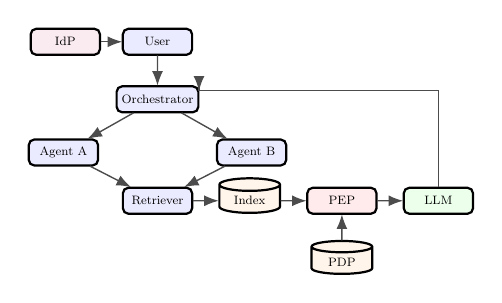
\begin{tikzpicture}[
    scale=0.55,
    transform shape,
    font=\footnotesize,
    node distance=0.6cm and 0.7cm,
    box/.style={draw, rounded corners=2pt, align=center, minimum width=16mm, minimum height=6mm, fill=blue!8, thick},
    cyl/.style={draw, cylinder, shape border rotate=90, aspect=0.3, align=center, minimum height=7mm, minimum width=14mm, fill=orange!8, thick},
    arr/.style={-Latex, line width=0.5pt, draw=black!70}
  ]
    \node[box, fill=purple!8] (IdP) {IdP};
    \node[box, right=0.5cm of IdP] (U) {User};
    \node[box, below=0.7cm of U] (O) {Orchestrator};
    \node[box, below left=0.6cm and 0.4cm of O] (A1) {Agent A};
    \node[box, below right=0.6cm and 0.4cm of O] (A2) {Agent B};
    \coordinate (Mid) at ($(A1)!0.5!(A2)$);
    \node[box, below=0.8cm of Mid] (R) {Retriever};
    \node[cyl, right=0.6cm of R] (I) {Index};
    \node[box, right=0.6cm of I, fill=red!8] (F) {PEP};
    \node[box, right=0.6cm of F, fill=green!8] (L) {LLM};
    \node[cyl, below=0.6cm of F] (P) {PDP};
    
    \draw[arr] (IdP) -- (U);
    \draw[arr] (U) -- (O);
    \draw[arr] (O) -- (A1);
    \draw[arr] (O) -- (A2);
    \draw[arr] (A1) -- (R);
    \draw[arr] (A2) -- (R);
    \draw[arr] (R) -- (I);
    \draw[arr] (I) -- (F);
    \draw[arr] (F) -- (L);
    \draw[arr] (P) -- (F);
    \draw[arr] (L) |- ([yshift=0.2cm]O.east) -- (O);
  \end{tikzpicture}
  \caption{Reference enforcement pattern that realizes AFR: the PEP gates retrieval candidates using the PDP before any chunk can enter any model context.}
  \label{fig:arch}
\end{figure}

\textbf{Key components:}
\begin{itemize}
  \item \textbf{IdP (Identity Provider)} authenticates users and provides verified identity claims.
  \item \textbf{Orchestrator} propagates user identity and scope to all agents.
  \item \textbf{Retriever} returns semantic pre-candidates (unfiltered).
  \item \textbf{PEP (Policy Enforcement Point)} queries the PDP, removes unauthorized chunks, and produces the authorized candidate set $\mathrm{cand}(q,u)$.
  \item \textbf{PDP (Policy Decision Point)} stores and evaluates authorization policies.
  \item \textbf{LLM} only sees authorized content.
\end{itemize}

%%%%%%%%%%%%%%%%%%%%%%%%%%%%%%%%%%%%%%%%%%%%%%%%%%%%%%%%%%%%%%%%%%%%%%%%%%%%%%%%
\section{Open Problems}
\label{sec:open-problems}

The comparative analysis shows a persistent gap: widely deployed stacks often lack AFR, inherited delegation enforcement, or isolation of shared retrieval-time state. The open problems below are organized around closing this gap while preserving practical latency and usability constraints.

\subsection{Research Challenges}

These problems require new theoretical frameworks or measurement approaches.

\textbf{Implicit leakage measurement.} How to quantify leakage through synthesis and inference when explicit chunks are filtered? This requires new metrics beyond chunk-level authorization, potentially drawing on differential privacy or information-theoretic notions.

\textbf{Embedding-level attacks.} Membership inference attacks~\cite{hayes2019mia} and vector database poisoning~\cite{zou2024poisonedrag} demonstrate that embeddings themselves carry security risks. Even if authorization filtering is correct, adversaries may poison the index or infer chunk membership from embedding distances. These attacks are orthogonal to but compounding with authorization failures.

\textbf{Attenuated delegation and the Confused Deputy.} Definition 2 inherits the full user scope $\mathrm{perm}(u)$ to all agents. This may violate least privilege and enables the classic \emph{Confused Deputy problem}: an agent performing a narrow task (e.g., calendar lookup) should not inherit the user's full HR data access, yet it may inadvertently invoke tools with broader scope. A refined model would use \emph{attenuated delegation}: $\mathrm{perm}(a_n) = \mathrm{perm}(u) \cap \mathrm{scope}(\mathrm{task}_n)$, where $\mathrm{scope}(\mathrm{task}_n)$ is the minimal permission set required for agent $a_n$'s current task. Defining and enforcing task-scoped permissions in agentic workflows, preventing agents from becoming confused deputies, is an open problem.

\subsection{Engineering Gaps Lacking Deployment at Scale}

These problems are well-understood conceptually but lack widely deployed solutions.

\textbf{Latency-security tradeoff at scale.} Enforcing AFR requires authorization checks on retrieval candidates before LLM access. For a typical top-100 retrieval with 1,000+ initial candidates, resolving RBAC permissions in under 100ms is a massive engineering hurdle. Pre-computation of user scope projections, batched authorization checks, and edge-cached permission graphs are potential directions, but we are not aware of published systems that demonstrate AFR at enterprise scale with end-to-end latency comparable to production RAG deployments.

\textbf{The broken chunk problem.} Naive chunking strategies split documents at fixed token boundaries. A single paragraph may contain both authorized and unauthorized information (e.g., ``Bob is on Project Alpha [public] and received a performance evaluation note [restricted]''). This creates partial-access failures where filtering the chunk loses authorized content, but including it leaks restricted content. Semantic chunking aligned with field-level authorization boundaries is an open problem.

\textbf{Delegation-aware auditing.} Agentic systems generate massive audit logs. A single user query may trigger dozens of agent invocations and thousands of authorization checks. Summarizing delegation chains into human-readable compliance reports is an open UX and systems question.

\textbf{Dynamic policy resolution and mid-conversation staleness.} In multi-agent RAG, a user's permissions may change mid-conversation. For example, temporary project access may expire, a role may be revoked, or a new sensitivity label may be applied to a document. If the PEP caches authorization decisions across turns, stale permissions can violate AFR even if the initial retrieval was correct. Conversely, re-querying the PDP on every turn introduces latency and may create inconsistent user experiences. Determining how to balance freshness, latency, and consistency in dynamic policy resolution remains an open systems challenge.

\textbf{Integration with existing policy engines.} How to adapt ReBAC/ABAC systems (OpenFGA, OPA, Zanzibar) for semantic retrieval workloads? These systems assume structured request-response patterns; vector similarity queries require new abstractions.

%%%%%%%%%%%%%%%%%%%%%%%%%%%%%%%%%%%%%%%%%%%%%%%%%%%%%%%%%%%%%%%%%%%%%%%%%%%%%%%%
\section{Related Work}
\label{sec:related}

\textbf{RAG.} Lewis et al.~\cite{rag} introduced RAG for knowledge-intensive tasks. Gao et al.~\cite{rag-survey} survey retrieval and generation but do not address authorization.

\textbf{Multi-agent orchestration.} AutoGen~\cite{autogen} and MetaGPT~\cite{metagpt} provide agent coordination abstractions but do not define authorization correctness.

\textbf{Prompt injection and defenses.} Greshake et al.~\cite{greshake2023indirect} and Liu et al.~\cite{liu2024ipi} study prompt injection risks. Hines et al.~\cite{hines2024spotlighting} propose spotlighting; Yi et al.~\cite{yi2025llmsecurity} benchmark defenses. These are complementary to authorization constraints: injection defenses protect model behavior, while authorization ensures data access control.

\textbf{Authorization engines.} OpenFGA~\cite{openfga} and Cerbos~\cite{cerbos} implement fine-grained authorization for structured requests. Google Zanzibar~\cite{zanzibar} pioneered relationship-based access control at scale. OPA~\cite{opa} provides policy-as-code for cloud-native environments. Semantic retrieval requires adaptation of these approaches.

\textbf{Cloud provider solutions.} AWS Bedrock~\cite{bedrock2025} provides metadata filtering and guardrails. This SoK evaluates these controls under AFR criteria.

\textbf{Vector security.} Hayes et al.~\cite{hayes2019mia} demonstrated membership inference attacks on generative model embeddings. Zou et al.~\cite{zou2024poisonedrag} showed vector database poisoning in RAG. Dwork et al.~\cite{dwork2006dp} established differential privacy foundations relevant to implicit leakage. These works address orthogonal but compounding risks.

\textbf{Access control foundations.} Sandhu et al.~\cite{rbac-original} and Ferraiolo and Kuhn~\cite{rbac-foundations} established RBAC theory.

\textbf{Relation to information flow control (IFC).} AFR shares conceptual lineage with IFC and taint tracking: both aim to prevent unauthorized information from influencing downstream computation. However, AFR is a weaker, more practical constraint. Full IFC would track information flow through all model parameters and intermediate states, which is intractable for current LLMs. AFR instead enforces an \emph{input-ordering constraint}: unauthorized information never enters the retrieval-to-generation pipeline. This is analogous to database inference control~\cite{denning1979tracker}, which prevents statistical queries from leaking individual records, but applied to semantic retrieval. We do not claim AFR subsumes IFC; rather, AFR is a deployable approximation for the RAG setting.

%%%%%%%%%%%%%%%%%%%%%%%%%%%%%%%%%%%%%%%%%%%%%%%%%%%%%%%%%%%%%%%%%%%%%%%%%%%%%%%%
\section{Conclusion}
\label{sec:conclusion}

Enterprise deployment of multi-agent RAG systems raises authorization questions that are not fully addressed by conventional access-control enforcement points. This SoK organized the problem space by defining threat models and correctness criteria, systematizing authorization failure modes, and classifying mitigation families.

We formalized Authorization-First Retrieval (AFR) as an ordering property that distinguishes defenses which constrain the semantic candidate space prior to downstream exposure from those that only filter after retrieval or generation. AFR-oriented architectures that resolve permissions at runtime against enterprise RBAC systems provide the strongest guarantees for authorization correctness and inherited delegation.

Our analysis suggests that without AFR, systems can at best provide behavioral non-disclosure rather than authorization correctness.

\section*{Acknowledgments}
[Omitted for blind review]

%%%%%%%%%%%%%%%%%%%%%%%%%%%%%%%%%%%%%%%%%%%%%%%%%%%%%%%%%%%%%%%%%%%%%%%%%%%%%%%%
% APPENDICES (per USENIX CFP: appear after main body, before references)
%%%%%%%%%%%%%%%%%%%%%%%%%%%%%%%%%%%%%%%%%%%%%%%%%%%%%%%%%%%%%%%%%%%%%%%%%%%%%%%%
\appendix

\section{Ethical Considerations}
\label{sec:ethics}

This work systematizes existing knowledge about authorization in RAG systems. It does not involve human subjects, datasets with personally identifiable information, or development of novel attacks. The failure modes and case studies presented are illustrative rather than exploits against deployed systems. No IRB approval was required.

\section{Open Science}
\label{sec:open-science}

This paper is a systematization; the primary artifact is the paper itself. To support reproducibility of the systematization claims, we provide an artifact package containing the raw data, reproducibility scripts, and classification rubrics used to derive Tables~\ref{tab:matrix} and~\ref{tab:systems}.

\textbf{Artifact contents.} The artifact package includes: (i) vendor documentation analysis worksheets summarizing authorization capabilities and limitations for each system evaluated, (ii) the scoring rubric used to derive guarantee ratings in Tables~\ref{tab:matrix} and~\ref{tab:systems}, (iii) system trace examples for each violation pattern (D3, D4, broad-retrieve-then-redact), and (iv) code snippets demonstrating each defense family's enforcement pattern.

\textbf{Reproducibility.} Running \texttt{make tables} regenerates Tables~\ref{tab:matrix} and~\ref{tab:systems} from the worksheets and rubric.

\textbf{Artifact availability.} The artifact package is available at the time of submission for peer review at: \url{https://anonymous.4open.science/r/agentic-rag-security-artifacts-4E40}

%%%%%%%%%%%%%%%%%%%%%%%%%%%%%%%%%%%%%%%%%%%%%%%%%%%%%%%%%%%%%%%%%%%%%%%%%%%%%%%%
\bibliographystyle{plainurl}
\begin{thebibliography}{99}

\bibitem{rag}
Lewis, P., Perez, E., Piktus, A., Petroni, F., Karpukhin, V., Goyal, N., K{\"u}ttler, H., Lewis, M., Yih, W., Rockt{\"a}schel, T., Riedel, S., and Kiela, D.
Retrieval-Augmented Generation for Knowledge-Intensive NLP Tasks.
\emph{Advances in Neural Information Processing Systems}, 33:9459--9474, 2020.

\bibitem{rag-survey}
Gao, Y., Xiong, Y., Gao, X., Jia, K., Pan, J., Bi, Y., Dai, Y., Sun, J., Wang, M., and Zhou, H.
Retrieval-Augmented Generation for Large Language Models: A Survey.
\emph{arXiv:2312.10997}, 2024.

\bibitem{bedrock2025}
Amazon Web Services.
Amazon Bedrock Knowledge Bases and Agents.
\url{https://aws.amazon.com/bedrock/}, 2024. Accessed: 2026-01-22.

\bibitem{autogen}
Wu, Q., Bansal, G., Zhang, J., Wu, Y., Li, S., Zhu, E., Jiang, B., Zhang, X., Wang, B., and Zhang, C.
AutoGen: Enabling Next-Gen LLM Applications via Multi-Agent Conversation.
\emph{arXiv:2308.08155}, 2023.

\bibitem{metagpt}
Hong, S., Zheng, X., Chen, J., Cheng, Y., Wang, C., Zhang, Z., Wang, Z., Zhang, P., Cai, G., and Ghita, M.
MetaGPT: Meta Programming for A Multi-Agent Collaborative Framework.
\emph{arXiv:2308.00352}, 2023.

\bibitem{greshake2023indirect}
Greshake, K., Abdelnabi, S., Mishra, S., Endres, C., Holz, T., and Fritz, M.
Not What You've Signed Up For: Compromising Real-World LLM-Integrated Applications with Indirect Prompt Injection.
In \emph{Proc. Workshop on AI and Security (AISec)}, 2023.

\bibitem{hines2024spotlighting}
Hines, K., Lopez, G., Hall, M., Peretti, F., and Palangi, H.
Defending Against Indirect Prompt Injection Attacks With Spotlighting.
\emph{arXiv:2403.14720}, 2024.

\bibitem{liu2024ipi}
Liu, Y., Jia, Y., Geng, R., Jia, J., and Gong, N.~Z.
Formalizing and Benchmarking Prompt Injection Attacks and Defenses.
In \emph{31st USENIX Security Symposium}, 2024.

\bibitem{yi2025llmsecurity}
Yi, J., Xie, Y., Zhu, B., Hines, K., Kiciman, E., Sun, G., Xie, Y., and Wu, F.
Benchmarking and Defending Against Indirect Prompt Injection Attacks on Large Language Models.
\emph{arXiv:2312.14197}, 2025.

\bibitem{openfga}
OpenFGA.
OpenFGA: Fine-Grained Authorization for Developers.
\url{https://openfga.dev}, 2024.

\bibitem{cerbos}
Cerbos.
Cerbos: The Open Source Authorization Layer for Applications.
\url{https://cerbos.dev}, 2024.

\bibitem{opa}
Open Policy Agent.
OPA: Policy-based Control for Cloud Native Environments.
\url{https://www.openpolicyagent.org}, 2024.

\bibitem{zanzibar}
Pang, R., Caceres, R., Burrows, M., Chen, Z., Dave, P., Germer, N., Golynski, A., Graney, K., Kang, N., Kissner, L., Korn, J.~L., Parmar, A., Richards, C.~D., and Wang, M.
Zanzibar: Google's Consistent, Global Authorization System.
In \emph{2019 USENIX Annual Technical Conference (USENIX ATC 19)}, pages 33--46, 2019.

\bibitem{rbac-original}
Sandhu, R.~S., Coyne, E.~J., Feinstein, H.~L., and Youman, C.~E.
Role-Based Access Control Models.
\emph{IEEE Computer}, 29(2):38--47, 1996.

\bibitem{rbac-foundations}
Ferraiolo, D.~F. and Kuhn, D.~R.
Role-Based Access Controls.
In \emph{15th National Computer Security Conference}, pages 554--563, 1992.

\bibitem{dwork2006dp}
Dwork, C., McSherry, F., Nissim, K., and Smith, A.
Calibrating Noise to Sensitivity in Private Data Analysis.
In \emph{Theory of Cryptography Conference (TCC)}, pages 265--284, 2006.

\bibitem{hayes2019mia}
Hayes, J., Melis, L., and Danezis, G.
LOGAN: Membership Inference Attacks Against Generative Models.
\emph{Proceedings on Privacy Enhancing Technologies (PoPETS)}, 2019(1):133--152, 2019.

\bibitem{zou2024poisonedrag}
Zou, W., Geng, R., Wang, B., and Jia, J.
PoisonedRAG: Knowledge Poisoning Attacks to Retrieval-Augmented Generation of Large Language Models.
\emph{arXiv:2402.07867}, 2024.

\bibitem{denning1979tracker}
Denning, D.~E., Denning, P.~J., and Schwartz, M.~D.
The Tracker: A Threat to Statistical Database Security.
\emph{ACM Transactions on Database Systems}, 4(1):76--96, 1979.

\end{thebibliography}

\end{document}
